%%%%%%%%%%%%%%%%%%%%%%%%%%%
% PREAMBOLO DEL DOCUMENTO %
%%%%%%%%%%%%%%%%%%%%%%%%%%%
\documentclass[a4paper,11pt,oneside,top=3cm,bottom=3cm,left=3.5cm,right=3.5cm,openright,reqno,table]{book}

% openany - fa iniziare i capitoli direttamente nella pagina successiva
% openright - fa iniziare i capitoli nella prima pagina destra disponibile 
% fleqn  - allinea le formule a sinistra anzichè centrarle
% leqno - dispone la numerazione delle formule sulla sinistra o destra
% reqno - dispone la numerazione delle formule sulla destra
%
\usepackage{packages}
% Per non appesantire troppo questo file
% quasi tutti i pacchetti usati sono salvati in packages.sty
%
\linespread{1.5}
% Per avere la parola BOZZA scritta su tutte le pagine

% funziona solo in modalità PS
% Invece per i PDF ho risolto così:
% pdftk tesi.pdf background bozza.pdf output tesi_bozza.pdf
%
%%%%%%%%%%%%%%%%%%%%%%%%%%%%%%%%%
%   DOCUMENTO VERO E PROPRIO    %
%%%%%%%%%%%%%%%%%%%%%%%%%%%%%%%%%
\begin{document}
% FRONTESPIZIO %
\begin{titlepage}
\changepage{}{}{}{-7.5 mm}{}{}{}{}{}
% parametri per cambiare le dimensioni di una singola pagina in ordine:
% {textheight}{textwidth}{evensidemargin}{oddsidemargin}{columnsep}
% {topmargin}{headheight}{headsep}{footskip}
% se voglio centrare la pagina devo mettere bindingoffset/2
% i primi 5 parametri posso usarli con \changetext


\begin{center}

\includegraphics [width=.15\columnwidth, angle=0]{unisa}\\ % height
\vspace{0.5cm}
{\LARGE \scshape Università degli Studi di Salerno}\\
\vspace{0.5cm}
{\Large Dipartimento di Informatica}\\
\vspace{0.1cm}
{\large Corso di Laurea Triennale in Informatica}\\
\vspace{1.5cm}
{\Large \scshape Tesi di Laurea} \\
\vspace{4cm}
{\Huge \bfseries \textsc{ShallWeGo}: AI-assisted mobility crowdsourcing platform} \\
\vspace{5cm}

\begin{minipage}[t]{7cm}
\flushleft
\textsc{Relatore}

Prof. \textbf{Fabio Palomba} \\
{\small Università degli studi di Salerno} \\[0.25cm]
\end{minipage}
\hfill
\begin{minipage}[t]{7cm}
\flushright
\textsc{Candidato}

\textbf{Hermann Senatore} \\
Matricola: 0512105743
\end{minipage}

\vspace{3cm}


{\small Anno Accademico 2020-2021}

\begin{comment}
\begin{table}[!h]
\centering
\begin{tabular}{c c c} %p{5cm}c
& Tesi di laurea & \\
& \textbf{Fabiano Pecorelli} & \\
& & \\[0.25cm]
Relatore \\
prof. \textbf{Andrea De Lucia} \\
{\small Università degli studi di Salerno} & & {\small Provincia di Salerno}\\
& & \\[0.5cm]
& {\small A.A. 2015-2016} & \\
\end{tabular}
\end{table}
\end{comment}
%
%
\end{center}

\end{titlepage}
%

\frontmatter
% quello che segue è in numerazione romana e i capitoli non verranno numerati
% se non si vuole che compaia il numero di pagina basta usare il comando:
%\nonumber

% RINGRAZIAMENTI %
\begin{titlepage}

\nonumber
\null \vspace {\stretch{1}}
	\begin{flushright}

	\textit{Il mondo è come un libro e chi non viaggia ne conosce una pagina soltanto.} \\
	\textit{\textbf{(Sant'Agostino)}}
	\end{flushright}



\end{titlepage}
% SOMMARIO %
\cleardoublepage
%\selectlanguage{italian}
\begin{abstract}
    La Tesi sviluppata si posiziona nell’ambito della creazione di strumenti informatici per assistere gli utenti del Trasporto Pubblico Locale nella loro esperienza quotidiana.
    L’obiettivo principale di questa Tesi consiste nello sviluppo di un’applicativo mobile che permetta l’accesso ad una piattaforma online chiamata \textsc{ShallWeGo} basata sulla collaborazione tra utenti che ha come scopo quello di consentire lo scambio di informazioni sull’organizzazione del Trasporto Pubblico Locale in una determinata zona. Il vero motore di \textsc{ShallWeGo} è quindi il singolo utente, che può mettere a disposizione la propria conoscenza sul topic in questione (organizzazione delle fermate sul territorio, aziende di trasporto e linee espletate da queste ultime) agli altri utenti, che quindi possono sopperire alle potenziali difficoltà di comunicazione da parte delle aziende di trasporto. Particolare attenzione deve essere dedicata tuttavia all’affidabilità di queste segnalazioni che devono essere controllate in qualche modo. È stato quindi previsto, tramite la definizione di un Agente Intelligente, un sistema di verifica delle segnalazioni anch’esso basato sulla partecipazione attiva degli utenti della piattaforma. Data una segnalazione sarà quindi possibile andare a determinare il gruppo di utenti che secondo determinate “metriche” risultino più adatti a verificarla e stabilire se quest'ultima possa essere integrata o meno sulla piattaforma.
\\[1cm]
\end{abstract} 
% INDICI %
\phantomsection
\addcontentsline{toc}{chapter}{Indice}
\tableofcontents
% Il simbolo * serve per evitare che comapaia nell'indice
\clearpage
%\listoffigures
%\clearpage
%\listoftables
% GLOSSARIO
%\cleardoublepage
\phantomsection
\addcontentsline{toc}{chapter}{Glossario}
% per inserire l'elenco dei simboli e degli acronimi nell'indice
\printglossary
% Per stampare il glossario
% per aggiornarlo si deve eseguire da terminale:
% makeindex -s myDoc.ist -t myDoc.alg -o myDoc.acr myDoc.acn
% per inserire una voce nell'elenco:
% \newglossaryentry{voce_etichetta}{name={voce}, description={descrizione}}
% se non compare direttamente nel testo va inizializzata con:
% \glsadd{voce_etichetta}
% oppure se viene richiamata all'interno del testo:
% \gls{voce_etichetta}
% SIMBOLI E NOTAZIONI %
\cleardoublepage
\phantomsection
\addcontentsline{toc}{chapter}{Elenco delle figure}
% per inserire l'elenco dei simboli e degli acronimi nell'indice
%\printglossary[type=\acronymtype,title=Elenco delle figure]
% Per stampare l'elenco dei simboli
\listoffigures
\cleardoublepage
\phantomsection
\addcontentsline{toc}{chapter}{Elenco delle tabelle}
% per inserire l'elenco dei simboli e degli acronimi nell'indice
%\printglossary[type=\acronymtype,title=Elenco delle figure]
% Per stampare l'elenco dei simboli
\listoftables
% per aggiornarlo si deve eseguire da terminale:
% makeindex -s myDoc.ist -t myDoc.glg -o myDoc.gls myDoc.glo
% per inserire una voce nell'elenco:
% \newglossaryentry{voce_etichetta}{name={voce}, description={descrizione}}
% se non compare direttamente nel testo va inizializzata con:
% \glsadd{voce_etichetta}
% oppure se viene richiamata all'interno del testo:
% \gls{voce_etichetta}

\mainmatter
% quello che segue sarà in numerazione araba e i capitoli verranno numerati
%\part{Studio iniziale}
% CAPITOLI
\phantomsection
%\addcontentsline{toc}{chapter}{Introduzione}
\chapter{Introduzione}
\markboth{Introduzione}{}
% [titolo ridotto se non ci dovesse stare] {titolo completo}

\section{Contesto applicativo e Motivazioni} %\label{1sec:scopo}
    \subsection{Lo stato del Trasporto Pubblico Locale}
    Negli ultimi due anni, complici anche gli avvenimenti che stanno interessando il mondo ed i successivi provvedimenti, le abitudini dei cittadini in tema di mobilità sono drasticamente cambiate.
    Tra i numerosissimi settori che sono interessati da questa ondata di cambiamenti ce n'è uno in particolare che ne ha risentito particolarmente: quello del Trasporto Pubblico Locale (\textbf{TPL}) che, secondo un rapporto stilato da varie associazioni di rappresentanza di aziende di trasporto presentato al Parlamento Italiano all'inizio del 2021 (\cite{statotpl}) e ripreso dal quotidiano "Il Sole 24 Ore" in data 25 Gennaio dello stesso anno (\cite{statotplsole24ore}) ha visto un crollo dei ricavi dell'entità dei Miliardi di Euro. Nello specifico, dal crollo della fruizione dei mezzi pubblici si stima che nelle casse delle aziende siano entrati complessivamente 250 milioni di Euro in meno al mese, portando le perdite complessive a circa 2 Miliardi.
    Tutto ciò, come anticipato, è causato sostanzialmente da un crollo delle presenza da parte dei cittadini su autobus, treni e metropolitane in un primo momento dovuto alle restrizioni imposte, almeno nel caso dell'Italia, nella prima metà del 2020 e complice la percezione da parte del cittadino dei mezzi pubblici come "poco sicuri" dal punto di vista sanitario risultando, continua il rapporto, in un calo del 90\% della domanda.
    Questi due fattori (crollo della domanda e conseguente diminuzione delle entrate) hanno generato in molti casi conseguenze pesanti sullo "stato di salute" delle aziende del settore, con successive rimodulazioni orarie e una sostanziale diminuzione delle corse, specie nelle prime e nelle ultime ore della giornata. La diminuzione delle corse inevitabilmente apre la porta ad uno dei problemi principali che sta affliggendo il settore nell'ultimo periodo: l'affollamento delle corse stesse.
    
    \subsection{Tecnologia e TPL}
    Con la sempre più capillare diffusione della tecnologia nelle mani del cittadino da un decennio a questa parte, i principali attori che operano in questo campo hanno riconosciuto l'importanza di andare a creare un sistema di informazione puntuale sul funzionamento del TPL in una determinata zona. Piattaforme come Google Maps, ad esempio, già da tempo forniscono dettagli sulla presenza di fermate e dettagli delle corse delle aziende di trasporto che operano in quella zona. 
    Nel caso particolare di Google Maps, questi dati, secondo la documentazione ufficiale del servizio "Google Transit" disponibile all'indirizzo \url{https://support.google.com/transitpartners/answer/1111471} sono ricavati principalmente dalle comunicazioni che giungono alla piattaforma da parte delle singole aziende che decidono di partecipare al programma, avendo poi l'opzione di condividere anche dati in tempo reale che permettano agli utenti di seguire in diretta l'andamento delle corse delle linee che gli interessano, tramite la piattaforma "Realtime Transit", che comunque è riservato alle aziende di trasporto.

    \subsection{Problemi delle attuali soluzioni}
    Come accennato in precedenza, i dati che sono disponibili sulle piattaforme più diffuse sono comunicati periodicamente dalle aziende che aderiscono a programmi come il sopracitato Google Transit su Maps. 
    Tuttavia, questo approccio non è esente da problemi di natura pratica: la presenza dei dati disponibili sulle varie piattaforme risulta quindi, nella maggior parte dei casi, essere subordinata all'adesione delle varie aziende. Se questo problema non si pone per le aziende di medie/grandi dimensioni che hanno a disposizione risorse economiche e tecnologiche, lo stesso non si può dire per le aziende più piccole che operanti solo in poche zone, che potrebbero avere difficoltà di carattere logistico anche solo nel posizionare gli adeguati segnali di riconoscimento delle fermate che utilizzano.
    Ne consegue quindi che gli utenti occasionali di queste aziende di trasporto (si pensi ad esempio ad una persona che si trova per la prima volta in una determinata zona) siano costretti a cercare informazioni presso altri cittadini che "ne sanno più di loro".
    Una piattaforma che ha provato a porre rimedio a questo problema è Moovit che ha lanciato nel 2015 un servizio chiamato "Mooviters' Community" che permette agli utenti di andare ad aggiungere dettagli alla piattaforma stessa che non siano stati già comunicati alle aziende. Questo approccio verrà trattato nel capitolo successivo dedicato proprio alle piattaforme presenti ad oggi sul mercato. 

\section{Obiettivi della tesi}
    L'obiettivo di questo lavoro è quindi proporre un primo esempio di soluzione ai due problemi di cui si è trattato in precedenza: creare una piattaforma, chiamata \textsc{ShallWeGo}, che metta a disposizione dei suoi membri gli strumenti adatti a diffondere la propria conoscenza in merito di organizzazione di linee e fermate nella loro zona con gli altri utenti, formando quindi una community che vede nella reciproca collaborazione il principale mezzo per raggiungere una vera e propria utilità per il singolo cittadino.

    
    
\section{Metodologie e risultati}
    \subsection{Approccio allo sviluppo della piattaforma}
        Lo sviluppo della piattaforma è cominciato, così come accade in tutti i progetti che prevedano la presenza di un software, con la raccolta e l'analisi dei requisiti, ovvero su \textit{cosa} dovesse fare la piattaforma. Una volta raccolti questi requisiti si è provveduto a categorizzarli in "prioritari" e "non prioritari". (Quelli individuati come prioritari sono stati elencati nella prima sezione del quarto capitolo). Ciò ha permesso di rendere chiaro sin da subito cosa risultasse più urgente realizzare per ottenere una prima versione funzionante della piattaforma. 
        Successivamente, si sono analizzate le varie strategie per lo sviluppo effettivo del software. Vista anche la distinzione tra requisiti "prioritari" e "non prioritari" appare palese come la strategia di sviluppo che più si adatta a questo contesto risulta quella \textbf{incrementale}. Lo sviluppo incrementale, nello specifico, consiste innanzitutto di implementare le funzionalità \textit{core} della piattaforma e, successivamente in modo \textit{incrementale} (e da qui la denominazione) tutte le varie funzionalità che vanno ad implementare i requisiti individuati in fase di analisi. 
        
        Le funzionalità \textit{core} prevedono l'impiego anche di due componenti particolari che non sono direttamente collegate con il software ma che sono necessarie per il corretto funzionamento dello stesso. Queste due componenti sono:
        \begin{itemize}
            \item Un server esterno per il geocoding, basato sull'applicativo Nominatim (per permettere un accesso semplice e veloce a dati geografici)
            \item Un modulo di intelligenza artificiale che permette la verifica di dati ottenuti dagli utenti.
        \end{itemize}

        Per quanto riguarda la componente descritta al primo punti, trattandosi di un software già realizzato e reso disponibile al pubblico tramite licenza \textbf{\textit{GNU Public License} 2.0}, non si può parlare di sviluppo ma di \textit{configurazione} o di \textit{tuning} per migliorare le prestazioni sulla macchina che lo ospita.

        \subsection{Perché l'Intelligenza Artificiale?}
            La componente di Intelligenza Artificiale descritta al secondo punto, invece, è stata quella verso la quale è stata posta la maggior parte dell'attenzione delle prime fasi di sviluppo. Ciò è giustificato dalla natura particolare della piattaforma, che permette agli utenti di essere la fonte di informazioni principale. Sorge quindi la necessità di prevedere un sistema molto veloce per la verifica (da parte di altri utenti, essendo la piattaforma \textit{community-driven}) della correttezza delle segnalazioni che pervengono alla piattaforma.  Un primo approccio a questo problema potrebbe essere rappresentato dalla semplice ricerca esaustiva dei candidati all'interno dell'insieme degli utenti. Quest'approccio risulta accettabile nel caso si consideri un dominio di utenti discretamente piccolo ma cessa di esserlo al crescere del numero di questi ultimi. È proprio in questo contesto che una tecnica di Intelligenza Artificiale si rivela essere adeguata: quella degli \textbf{Algoritmi Genetici}. L'idea che sta alla base degli Algoritmi Genetici ricalca a grandi linee (come d'altronde suggerisce il nome) quello dell'evoluzione di una popolazione di individui (un insieme di soluzioni ad un problema) descritta per la prima volta da Charles Darwin nel 1859 nella sua opera "L'Origine della Specie", che si compone di tre "tappe" principali, ripetute moltissime volte:

            \begin{itemize}
                \item \textbf{Selezione};
                \item \textbf{Crossover} o \textbf{Accoppiamento} degli individui;
                \item \textbf{Mutazione} degli individui.
            \end{itemize}

            Questo processo permette di ottenere, con il susseguirsi delle \textit{generazioni}, una popolazione composta da individui molto forti che si adattano ai vari cambiamenti nell'ambiente in cui si trovano.
            Allo stesso modo, a partire da un insieme iniziale di soluzioni ad un problema, tramite un Algoritmo Genetico è possibile ottenere in maniera molto veloce (come risulta necessario nel caso della piattaforma in sviluppo) delle soluzioni ammissibili che risultino almeno "buone" per il problema che si sta affrontando. Non trattandosi di una ricerca esaustiva, tuttavia, non è garantito il raggiungimento della soluzione ottima.

            Il funzionamento dell'Algoritmo Genetico sviluppato per \textsc{ShallWeGo} verrà descritto in dettaglio nel \textbf{Terzo Capitolo} che è dedicato interamente a questo \textit{topic}.

        \subsection{Il problema delle API}
            L'applicazione oggetto di questo lavoro di Tesi fa largo uso di mappe e dati geografici in generale. Google Maps mette a disposizione le sue API in maniera gratuita fino ad esaurimento di un credito (che viene scalato man mano che si utilizzano i propri servizi) che si rinnova ogni mese. Superata questa soglia, è necessario sostenere un certo prezzo.
            Le tariffe, consultabili all'indirizzo \url{https://cloud.google.com/maps-platform/pricing}, prevedono infatti la possibilità di usufruire un credito gratuito dell'entità di 200\$ mensili. In particolare, il servizio di Geocoding \footnote[1]{Ovvero il processo che consente di ottenere il nome logico di un luogo associato ad una coppia di coordinate (Latitudine, Longitudine) e viceversa} costa 5\$ ogni 1000 richieste. Il prezzo, quindi, aumenta all'aumentare delle richieste che vengono effettuate da chi utilizza l'applicazione.
            Sono tuttavia disponibili delle alternative di terze parti che permettono l'accesso gratuito a degli endpoint per effettuare le operazioni di Geocoding. Uno dei migliori servizi di questo genere è rappresentato da \textbf{Nominatim} che è utilizzato, tra l'altro, anche dal progetto \textbf{OpenStreetMap} per implementare la feature di ricerca nella loro piattaforma. Il funzionamento di Nominatim verrà descritto in dettaglio nel \textbf{Quarto Capitolo} della Tesi che tratta l'architettura ed il funzionamento di \textsc{ShallWeGo}.
    
    \subsection{Risultati ottenuti}
        Il risultato di questa esperienza di Tesi è stato quindi quello di aver sviluppato una prima versione di un applicativo mobile e della relativa componente server che implementasse l'idea di cui si è discusso. L'applicativo consiste in un semplice file .apk per Android installabile e che, attualmente, previa registrazione ed ottenimento di uno username, permetta a chi vuole di cominciare ad effettuare segnalazioni riguardanti fermate, linee ed aziende di trasporti che conosce e che sa operare in una determinata zona.
        È presente anche una feature che prevede la possibilità da parte di un utente di comunicare in tempo reale la propria posizione e, contemporaneamente, specificare su che linea si trova, così da permettere ad altri utenti interessati di farsi un'idea di quanto debbano aspettare per salire a bordo.
        
        \newpage

\section{Struttura della tesi}
        La tesi è strutturata principalmente in cinque parti, che coprono gli aspetti principali del lavoro svolto, con un'attenzione particolare alla metodologia utilizzata per implementare in modo efficiente la valutazione delle segnalazioni che pervengono alla piattaforma da parte degli utenti. \\
        In particolare:
        \begin{itemize}
            \item Il Primo Capitolo funge da introduzione al lavoro svolto per realizzare la piattaforma;
            \item Il Secondo Capitolo descrive le principali soluzioni che sono attualmente utilizzabili dagli utenti per quanto riguarda il dominio del problema trattato dal lavoro di Tesi;
            \item Il Terzo Capitolo descrive accuratamente l'approccio usato per la valutazione delle segnalazioni degli utenti, che fa uso di una tecnica di \textbf{Intelligenza Artificiale} e che permette di selezionare gli utenti più adatti a valutare una determinata segnalazione;
            \item Il Quarto Capitolo, invece, illustra l'architettura su cui si basa l'applicazione e i dettagli implementatiti in termini di framework, linguaggi di programmazione e librerie di terze parti utilizzate per lo sviluppo dell'applicativo mobile;
            \item Infine, il Quinto Capitolo riassume tutti gli sviluppi futuri che permetterebbero all'applicazione di uscire dallo stato di "demo" ed essere quindi messa a disposizione del pubblico.
        \end{itemize}

\chapter{Stato dell'arte} %\label{1cap:spinta_laterale}
% [titolo ridotto se non ci dovesse stare] {titolo completo}
%

\begin{citazione}
    \textit{Lo scopo di questo capitolo è di illustrare la situazione attuale dei vari applicativi che sono a disposizione degli utenti del trasporto pubblico locale (TPL) per permettergli di organizzare i loro spostamenti.}
\end{citazione}

\newpage

I principali attori sul panorama della diffusione di informazioni sul TPL sono senz'altro la piattaforma Maps di Google ed in particolare Moovit, che ha acquisito una maggiore popolarità nell'ultimo anno.

\section{Google Maps}
    Transit è un servizio messo a disposizione da Google ed integrato nella piattaforma Maps che consente all'utente di visualizzare le informazioni \textit{statiche} messe a disposizione dalle varie aziende di trasporto tramite il programma "Google Transit Partners", che quindi consistono nella programmazione giornaliera delle corse e dell'organizzazione delle fermate sul territorio in questione. \\
    Oltre ai dati statici, le aziende di trasporto possono condividere con Google mediante la piattaforma \textbf{Realtime Transit} che quindi permette di visualizzare all'interno di Maps i dati in tempo reale sulla posizione dei mezzi pubblici in un determinato istante. Questa funzionalità, così come tutti i dati relativi al trasporto pubblico su Maps sono disponibili solo su iniziativa delle aziende che decidono di partecipare al programma. Un esempio di azienda che mette a disposizione i dati realtime è per esempio l'ATAC di Roma, che li offre a partire da Settembre 2019 (\cite{atactransit})  \\
    I dati (siano essi statici o dinamici) sono comunicati a Google su base regolare dalle aziende (tipicamente settimanale, secondo quanto riportato nella sezione FAQ della pagina dedicata \footnote[3]{\url{https://developers.google.com/transit/gtfs/guides/faq}}) tramite il formato GTFS \textit{(General Transit Feed Specification)} che permette di strutturare in maniera efficiente i dati riguardanti il trasporto pubblico.

    Esistono due "varianti" del formato GTFS:
    \begin{itemize}
        \item \textbf{GTFS Statico}, che raccoglie i dati "statici" (quindi gli orari previsti delle corse e l'organizzazione delle fermate sul territorio)
        \item \textbf{GTFS Realtime}, che raccoglie i dati "dinamici" (come l'andamento delle corse in tempo reale)
    \end{itemize}

    Tuttavia, come accennato in precedenza, questi dati sono comunicati su richiesta delle aziende e solo un numero limitato di queste ultime (almeno in Italia) aderisce al programma, limitando così i dati a disposizione dell'utente.

\section{Mobilità e crowdsourcing}
    La tecnica del crowdsourcing, applicabile nella maggior parte dei casi in cui ci sia bisogno di ottenere dati di interesse per un determinato dominio consiste nel ricavare direttamente questi ultimi da persone sul campo e che ritengano di possedere un'informazione che potrebbe tornare utile alla comunità.
    Anche nel dominio di interesse della piattaforma che si vuole sviluppare, è possibile andare ad isolare i dati di interesse (quelli utili cioè a fornire un sufficiente livello di informazione agli utenti del TPL). Possono essere riassunti in cinque punti:
            \begin{itemize}
                \item Posizione di una fermata in un determinato punto
                \item "Equipaggiamento" di una fermata (in termini di pensilina, segni identificativi e quadri orari disponibili al pubblico)
                \item Utilizzo di una fermata da parte di una determinata linea
                \item Destinazioni di una linea
                \item Eventi transitori (come presenza di traffico, avvisi su deviazioni o strade chiuse)
            \end{itemize}

        L'approccio del crowdsourcing è già utilizzato sia in Google Maps (di cui si è appena parlato) sia in un'altra piattaforma che risulta di particolare interesse, ovvero \textbf{Moovit}. Moovit sfrutta l'idea del crowdsourcing per ottenere dati altrimenti molto difficili da reperire.

    \subsection{La Community di Moovit: un caso di studio}
        Moovit è una piattaforma che al contrario di Google Maps si occupa esclusivamente di mobilità.
        Nasce nel 2012 e nel 2015 viene acquistata da Intel. Attualmente Moovit si sta impegnando per sviluppare soluzioni di Mobility as a Service.
        Il Mobility as a Service (MaaS) è un concetto relativamente nuovo, che permette all'utente di scegliere il modo che ritiene più adatto di spostarsi (tramite mezzi pubblici, car sharing e simili) usando una sola piattaforma che mette a disposizione tutti questi servizi, favorendo quindi l'interoperabilità tra i vari mezzi di trasporto. \\

        Dal 2015, inoltre, Moovit mette a disposizione un servizio chiamato \textbf{Mooviter Community}, che permette al singolo utente della piattaforma di partecipare alla mappatura delle fermate e delle linee della sua zona tramite un Editor accessibile via web. I cambiamenti dovranno quindi essere approvati dagli amministratori della piattaforma o da utenti esperti. \\

        In particolare, la piattaforma di Moovit organizza gli utenti in "livelli", che potranno essere "scalati" man mano che si matura esperienza in termini di segnalazioni. Nello specifico, se un utente $x$ di livello $n$ effettua una segnalazione, chi potrà verificare questa segnalazione sarà solamente un certo utente $z$ il cui livello risulta almeno $n + 1$ o che sia membro del Team. \\
        Il problema di questo approccio è che se un utente con molta esperienza si unisce alla piattaforma in un certo momento, egli non potrà immediatamente cominciare a verificare segnalazioni poiché inizialmente il suo livello sarà troppo basso.\\
        Attualmente, l'Editor della Community di Moovit è disponibile in tutte le sue funzionalità esclusivamente via web tramite un browser che riporta uno \textit{user-agent} desktop. \\

        Oltre all'editor delle fermate e delle linee, nell'ultimo periodo Moovit ha messo a disposizione direttamente dall'app mobile uno strumento che permette di segnalare anche l'affollamento di una determinata corsa, come riportato sul sito web della piattaforma.\footnote[4]{\url{https://moovit.com/press-releases/moovit-crowding-report/}}

\newpage
\section{Il focus di ShallWeGo}
    La piattaforma ShallWeGo si basa principalmente sul modello delineato da Moovit con la sua Community rendendo tuttavia i dati ottenuti direttamente dagli utenti la fonte principale di informazioni, fornendo gli strumenti adatti per rendere disponibili i dettagli sulle aziende, sulle corse e sulle fermate in una determinata zona tramite un'applicazione mobile che ne semplifichi l'accessibilità anche all'esterno in quanto, come accennato in precedenza, la piattaforma di Moovit risulta principalmente web-based, separata dall'applicazione principale che è più conosciuta al grande pubblico. \\
    Inoltre, a differenza della Community di Moovit, in ShallWeGo le segnalazioni non sono limitate solamente a dettagli statici ma si estendono anche ad eventi "dinamici" (come strade chiuse, deviazioni, traffico o incidenti), ai dettagli di una singola fermata (come l'affollamento, la presenza di pensiline, di paline di riconoscimento delle aziende che la utilizzano o dei quadri orari) ed all'andamento delle corse, sfruttando il dispositivo dell'utente, permettendo quindi ad altri membri della community di verificare la presenza e la posizione di una corsa nell'ambito di una linea, in modo simile a quanto avviene con Transit Realtime di Google, ma con la differenza che non risulta necessario che le aziende condividano i dati. La feature presente in ShallWeGo permette anche di condividere informazioni sulla corsa stessa quali l'affollamento, la temperatura o le condizioni del mezzo in quel momento (come ad esempio lo stato di funzionamento delle obliteratrici o dell'aria condizionata) \\
    Infine, dal punto di vista della verifica delle segnalazioni, ShallWeGo non possiede un team che si dedica a valutare le segnalazioni, ma al contrario i verificatori più adatti vengono scelti mediante una componente di Intelligenza Artificiale creata proprio a questo scopo ed integrata nell'infrastruttura dell'applicazione. In particolare, l'Algoritmo per la scelta degli utenti si basa, oltre che sull'esperienza accumulata sulla piattaforma da parte di un singolo (in termini di segnalazioni effettuate e valutate) anche sulla distanza geografica dell'area in cui egli opera dal luogo della segnalazione. In questo modo, anche i nuovi iscritti alla piattaforma avranno la possibilità di valutare le segnalazioni inviate alla piattaforma. I dettagli sul funzionamento della componente di Intelligenza Artificiale saranno discussi nel capitolo successivo.
\chapter{Background sull'Intelligenza Artificiale utilizzata} %\label{1cap:spinta_laterale}
% [titolo ridotto se non ci dovesse stare] {titolo completo}
%

\begin{citazione}
    \textit{Lo scopo di questo capitolo è di illustrare in dettaglio la componente di Intelligenza Artificiale che orchestra la verifica delle segnalazioni. In particolare, si descrive l'idea generale che sta alla base degli Algoritmi Genetici e viene proposta una panoramica delle operazioni tipiche di questo paradigma che includono quelle di Selezione, di Crossover e di Mutazione. Viene inoltre proposta una panoramica sulle operazioni di postprocessing effettuate dopo il termine dell'algoritmo.}
\end{citazione}

\newpage

\section{Descrizione del problema da affrontare}
    Come descritto in precedenza, la fonte dei dati disponibili in \textsc{ShallWeGo} risiede nella sua community di utenti, che mettono a disposizione la loro conoscenza del \textit{topic} con gli altri. Il concetto base su cui si basa la piattaforma è quindi la \textbf{segnalazione} da parte del singolo. Di questi dati, non essendo forniti direttamente dalle aziende di trasporto, non è però garantita la precisione o addirittura la correttezza. Sorge quindi il bisogno di effettuare una qualche tipo di \textbf{validazione}. \\
    Gli utenti più adatti a validare i dati di una certa segnalazione sono quelle che possiedono principalmente i seguenti requisiti:
    \begin{itemize}
        \item Risiedano (oppure operino abitualmente) in una zona vicina al luogo oggetto della segnalazione;
        \item Abbiano una certa "reputazione" all'interno della piattaforma. (\textsc{ShallWeGo} infatti tiene traccia del livello di attività in termini di segnalazioni e di verifica delle stesse. Questo livello, similmente a quanto avviene sul social network \textbf{Reddit}, viene chiamato "\textit{karma}" e cresce all'aumentare dell'attività del singolo).
    \end{itemize}

    I "verificatori" sono assegnati all'atto dell'invio di una segnalazione da parte dell'utente. 
    Se ci si pone nello scenario in cui la piattaforma cresce in termini di numero di utenti, una ricerca esaustiva all'interno dell'insieme degli iscritti per assegnare quelli più adatti risulta essere problematica dal punto di vista della complessità. Si è quindi deciso di sfruttare una tecnica particolare che permetta di ridurla: quella degli \textbf{Algoritmi Genetici}, particolarmente utili alla ricerca in domini molto grandi.

\section{Algoritmi genetici}
    Quella degli algoritmi genetici (\textbf{GA}) è una \textbf{metaeuristica}, ovvero una serie di euristiche che, combinate, consentono di implementare un algoritmo di \textbf{ricerca} per risolvere problemi di ottimizzazione. In quanto metaeuristica, il paradigma che sta alla base degli algoritmi generici non garantisce di trovare la soluzione ottima nello spazio di ricerca che si sta considerando ma permette di trovare in maniera molto veloce (e in questo risiede uno dei suoi vantaggi che lo fanno preferire ad altri approcci) delle soluzioni che vi si avvicinano. Un altro vantaggio che rende molto utile l'impiego di algoritmi che si basano su questa metaeuristica, consiste nel fatto che essi siano sempre applicabili, a prescindere dalla struttura del problema. \\
    In particolare, ad un algoritmo che sfrutta questa metaeuristica viene presentato un insieme iniziale di soluzioni ammissibili al problema che si sta affrontando e, secondo determinate metriche che forniscono una stima di quanto \textit{"buona"} sia una certa soluzione a quel determinato problema, stabilire la migliore (o le migliori), andando a crearne di nuove se necessario.

\section{Struttura e funzionamento generale degli algoritmi genetici}
    In generale, il funzionamento degli algoritmi genetici (e da qui la denominazione del paradigma) ricalca a grandi linee quella dell'evoluzione delle specie descritte da Charles Darwin nel 1854 nella sua opera \textit{"L'origine della specie"} per cui l'evoluzione delle specie presenti in natura segue un cammino ben preciso, che consiste in tre fasi ben precise, a partire da una popolazione iniziale di individui:

    \begin{itemize}
        \item Selezione naturale;
        \item Accoppiamento tra individui (detto anche, nel contesto che si sta trattando, \textit{crossover});
        \item Mutazione di un gene di un individuo.
    \end{itemize}

    Un individuo, secondo quanto descritto da Darwin, può essere visto come un insieme di caratteristiche (o \textit{geni}) che ne definiscono l'identità. Mediante l'accoppiamento, i geni di due individui si mescolano e vanno a creare un altro individuo che possiederà quindi una combinazione di quelli dei suoi genitori. \\
    Con una certa probabilità, inoltre, avviene il fenomeno della mutazione, descritto poc'anzi.

    Infine, sulla base di quanto buone siano le caratteristiche di un individuo, esso potrà "sopravvivere" ed eventualmente riprodursi per formare nuovi individui o "morire", non propagando oltre i suoi geni, che evidentemente non lo rendevano abbastanza adatto all'ambiente in cui si trovava. Il processo quindi risulta \textit{iterativo}.

    La strategia utilizzata da un algoritmo che implementa questo paradigma è particolarmente simile a quella descritta da Darwin per il suo campo di studi.

    Portando avanti la similitudine con quanto avviene in natura, quando si vuole affrontare un dato problema (che chiameremo $x$) mediante la tecnica degli algoritmi genetici innanzitutto vengono generate in maniera più o meno casuale una serie di soluzioni ammissibili per $x$ (gli \textit{individui}), ognuna di loro composta da differenti caratteristiche (i \textit{geni} dell'individuo). Questo insieme di soluzioni al problema rappresenta la cosiddetta \textbf{popolazione iniziale}. A partire da quest'ultima, viene solitamente calcolato l'indice di "bontà" di ogni singola soluzione (che in gergo viene chiamata \textbf{fitness}), tramite una funzione apposita, chiamata appunto \textbf{\textit{funzione di Fitness}}. Una volta valutata questa quantità è necessario stabilire a quanti e a quali individui sia concesso riprodursi. \\
    Per questa ragione, a questo stadio si affronta solitamente la fase di \textbf{selezione}, che consiste nel far sopravvivere solamente gli individui migliori in termini di fitness. Gli individui che sopravvivono alla selezione sono ammessi al cosiddetto \textbf{mating pool}, ovvero saranno membri dell'insieme degli individui che si possono riprodurre. \\
    Una volta effettuato l'accoppiamento, la popolazione risultante è rappresentata da un nuovo insieme di individui che, come accennato in precedenza, posseggono una parte dei geni del primo genitore ed una parte dei geni del secondo, mutuandone quindi le loro caratteristiche. \\
    Si passa poi all'ultimo stadio dell'evoluzione, in cui avviene (con una certa probabilità) la \textbf{mutazione} di uno o più geni che compongono un individuo all'interno della popolazione. \\
    A questo punto l'algoritmo si trova davanti ad una scelta: 
    \begin{itemize}
        \item Ricominciare dall'operazione di selezione usando come popolazione quella risultante dall'operazione di mutazione;
        \item Terminare il processo.
    \end{itemize}

    Per prendere una decisione, l'algoritmo fa riferimento alla cosiddetta \textbf{condizione di terminazione}, che rappresenta le condizioni che si devono verificare per mettere fine al processo (come ad esempio il numero di iterazioni effettuate, il tempo di esecuzione o il peggioramento in termini di fitness media della popolazione dopo un numero $n$ fissato di iterazioni). Se la condizione di terminazione viene soddisfatta, allora il processo giunge al termine e solitamente viene restituito l'individuo migliore in termini di fitness dell'ultima popolazione, al netto di accorgimenti particolari e di operazioni di post-processing.

    Le operazioni di selezione, crossover e mutazione vengono implementate tramite procedure chiamate \textbf{operatori genetici}, la cui definizione rappresenta uno degli step più importanti dell'implementazione di un algoritmo di ricerca che sfrutta questa metaeuristica, assieme a stabilire come debba essere calcolata la fitness e come e quando debba terminare il processo. 

    \newpage

\section{L'algoritmo utilizzato da \textsc{ShallWeGo}}
    In questa sezione verrà descritto accuratamente l'algoritmo di ricerca utilizzato dalla piattaforma che segue il paradigma degli algoritmi genetici e che va a risolvere il problema di ottimizzazione consistente nel selezionare i migliori potenziali verificatori di una determinata segnalazione.

\subsection{Codifica dell'Individuo}
    Nell'algoritmo presente in \textsc{ShallWeGo}, si definisce individuo un insieme di 5 utenti. Nella popolazione iniziale gli utenti che compongono gli individui sono presi in maniera casuale da quelli che operano nella provincia della segnalazione. In questo modo, sfruttando la vicinanza territoriale, viene aumentata la possibilità che questi utenti siano a conoscenza dell'oggetto della segnalazione per la quale sono stati scelti. La distanza tra il luogo della segnalazione e quello in cui opera l'utente viene calcolata effettuando delle operazioni di geocoding tramite il server Nominatim messo a disposizione per l'occasione. Questo aspetto verrà trattato in dettaglio nel capitolo dedicato all'architettura della piattaforma. Il numero di individui inseriti nella popolazione iniziale è fissato a \textbf{50}.

\subsection{Funzione di Fitness}
    All'inizio di questo capitolo, è stato delineato l'\textit{identikit} del verificatore ideale per una certa segnalazione. Le metriche utilizzate, riassumendo, sono:

    \begin{itemize}
        \item La distanza in chilometri tra il luogo di una segnalazione e l'area in cui opera un utente;
        \item La "reputazione" (o karma) che un utente si è costruito durante la sua permanenza sulla piattaforma.
    \end{itemize}

    Dal punto di vista matematico, la funzione di fitness può essere formalizzata in questo modo, se $x$ rappresenta il valore (chiaramente $>=$ 0) in chilometri della distanza ed $y$ il valore di karma dell'utente:

    \[ f(x, y) =
  \begin{cases}
    \frac{4(250 + \frac{100}{x+0,3}) + 2y}{2}      & \quad \text{se } x \text{ < 15}\\
    \frac{4(\frac{30}{x})^2 + 2y}{2}  & \quad \text{altrimenti}
  \end{cases}
\]

\newpage
La struttura dell'equazione conferma quanto accennato poc'anzi sul dare la priorità alla distanza geografica piuttosto che (almeno in un primo momento della vita della piattaforma, con una distribuzione più uniforme degli utenti) al karma. Infatti, un utente che opera in un'area che dista meno di \textbf{15km} dal luogo della segnalazione ha intuitivamente più probabilità di essere a conoscenza della struttura della rete di trasporti in quella zona (e quindi risulta più adatto al ruolo di verificatore). \\
Ed infatti, visto l'andamento della funzione $f(x) = \frac{100}{x}, x \neq 0$ (il cui andamento è mostrato nella figura successiva e che a valori piccoli di $x$ associa valori grandi di $f(x)$) e vista la presenza della costante additiva (250), un utente che opera in quel range di distanza dalla segnalazione risulta molto forte agli occhi dell'algoritmo.
\begin{figure}[h!]
    \begin{center}
        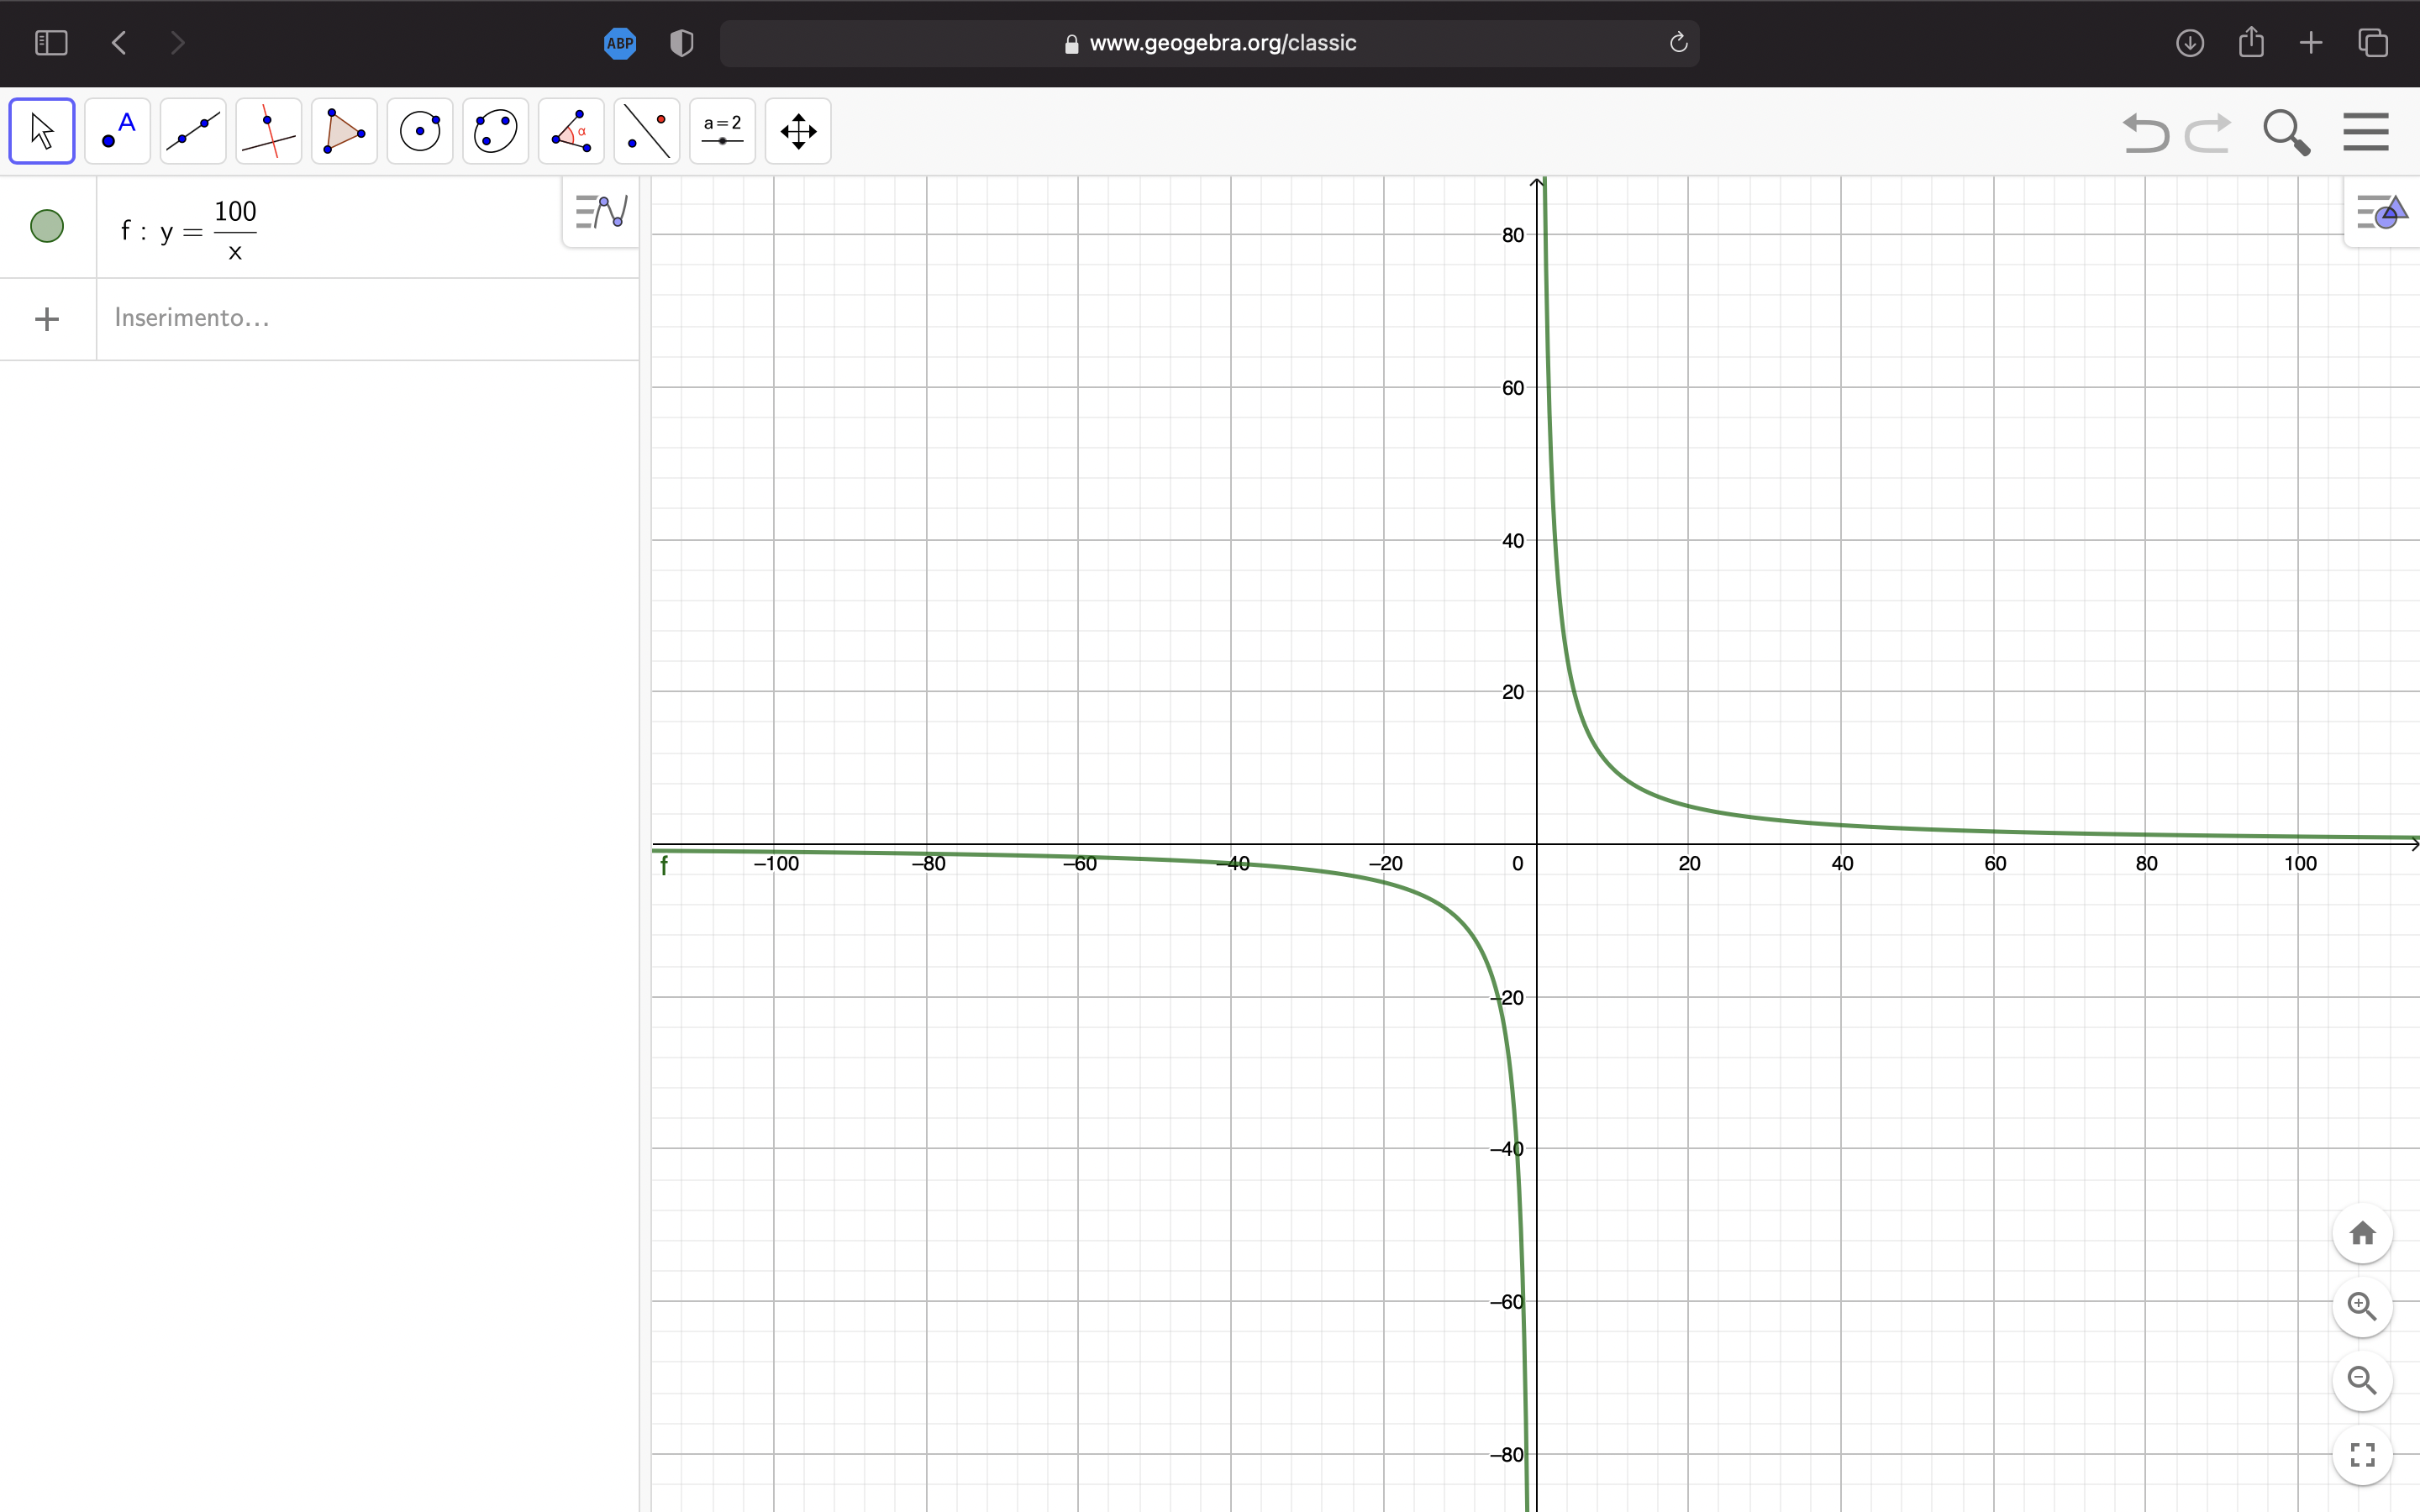
\includegraphics[scale=0.30]{100x}
    \end{center}
    \caption{L'andamento della funzione $100/x$}
    \label{fig: L'andamento della funzione $100/x$}
\end{figure}

La fitness di un determinato individuo, al contrario di quanto accade in altri tipi di algoritmi genetici, viene calcolata effettuando la \textbf{media aritmetica} della fitness di ogni gene all'interno dell'individuo. 
\newpage
\section{Operatori genetici}
  Verranno ora illustrate le scelte che sono state prese riguardo l'implementazione dei vari operatori genetici che prendono parte al processo di evoluzione tipico degli algoritmi genetici. Tutte le metodologie introdotte in questa sezione sono state illustrate nella sesta lezione del corso di \textit{Fondamenti di Intelligenza Artificiale} tenuta dal Prof. \textbf{Fabio Palomba} e dal Dott. \textbf{Emanuele Iannone} nell'anno 2020.

    \subsection{L'operatore genetico di Selezione}
        Il primo operatore che viene applicato in una singola iterazione dell'algoritmo è quello di \textbf{Selezione}, che, riprendendo quanto descritto in precedenza, permette di stabilire a quali individui sia concesso riprodursi sulla base della loro fitness. In letteratura, esistono diversi approcci che possono essere seguiti per realizzare quest'operazione. \\
        Tra questi vanno menzionati in particolare:

        \begin{itemize}
            \item L'approccio basato su \textbf{roulette wheel}, in cui gli individui con la fitness più alta hanno più possibilità di sopravvivere, proprio come succede ad un elemento posto su una roulette che ha una porzione di area maggiore rispetto agli altri. In questo caso, la "porzione" di roulette dedicata ad ogni individuo sarà direttamente proporzionale al valore della sua fitness (normalizzata in $[0, 1]$);
            \item L'approccio basato su \textbf{rank}, nel quale ogni individuo della popolazione è ordinato in modo decrescente rispetto alla sua fitness e ad ogni posizione in questa lista viene associato un numero, il cosiddetto \textit{rango}: la probabilità di selezione del singolo risulta inversamente proporzionale al suo rango;
            \item L'approccio basato su \textbf{truncation}, in qualche modo simile al precedente (ne mutua l'ordinamento degli individui) che consiste nel fissare un numero $n$ < $|P|$ (se P rappresenta la popolazione) e di selezionare i primi $n$ individui nella popolazione che hanno la fitness più alta.
        \end{itemize}

        Per l'algoritmo utilizzato in \textsc{ShallWeGo} si è scelto di utilizzare l'approccio basato su \textbf{roulette wheel} in quanto risulta quello di più immediata comprensione ed implementazione (essendo molto più fedele a quanto avviene in natura). Inoltre, non essendoci alcun caso in cui la fitness possa scendere sotto il valore $0$ quest'approccio è stato applicabile senza problemi.

    \subsection{L'operatore genetico di Crossover}
        Dopo l'applicazione dell'operatore di Selezione (e quindi con la definizione di quelli che sono i componenti del cosiddetto \textbf{mating pool}), si procede con la fase di \textbf{crossover}, che prevede l'accoppiamento di coppie di individui all'interno del mating pool. 
        Esistono diverse tecniche che permettono di implementare questa operazione. \\
        Tra queste si menzionano:

        \begin{itemize}
            \item La tecnica \textbf{Single Point} che dati due individui x = ($x_{0}, x_{1}, ..., x_{n}$) ed y = ($y_{0}, y_{1}, ..., y_{m}$), prevede la creazione di due nuovi individui $j$ e $k$ che siano il risultato di un incrocio tra i geni dei loro genitori, dopo aver selezionato il cosiddetto \textbf{punto di taglio}, ovvero quel punto $z$ tale che:
                \begin{itemize}
                    \item $j = x_{0}, x_{1}, ..., x_{z}, y_{z+1}, ..., y_{m}$ e
                    \item $k = y_{0}, y_{1}, ..., y_{z}, x_{z+1}, ..., x_{n}$
                \end{itemize}
            \item La tecnica \textbf{\textit{k}-points}, che rappresenta una generalizzazione della tecnica Single Point, in cui un individuo viene diviso in \textit{$k$} porzioni prima di essere incrociato con un altro individuo;
        \end{itemize}
        La tecnica usata da \textsc{ShallWeGo} è quella del \textbf{Single Point}. C'è da precisare che nel caso del problema che si sta affrontando la posizione di un gene all'interno di un individuo risulta irrilevante e di conseguenza un approccio k-points non avrebbe portato a nessun tipo di miglioramento.
    \subsection{L'operatore genetico di Mutazione}
        L'ultimo operatore genetico che viene applicato durante un'iterazione è quello di \textbf{Mutazione} che ricalca, come accennato precedentemente, il processo di mutazione spontanea che avviene in natura. Una mutazione consiste nel cambiamento casuale di un gene all'interno di un individuo. Anche in questo caso, esistono diversi approcci che in generale possono essere seguiti. \\
        Tra questi si menzionano:
        \begin{itemize}
            \item La tecnica del \textbf{Bit Flip} che, come suggerisce il nome, è applicabile solo nel caso di individui codificati in modo \textit{binario} e consiste nel scegliere in maniera casuale un gene all'interno dell'individuo e "capovolgere" il suo valore (quindi da 0 si passa ad 1 e viceversa);
            \item La tecnica del \textbf{Random Resetting} che prevede il cambiamento di un gene preso casualmente all'interno dell'individuo con un altro valore ammissibile per quel gene preso altrettanto casualmente;
            \item La tecnica dello \textbf{Swap} che prevede lo scambio di due geni all'interno dell'individuo;
            \item La tecnica dello \textbf{Scramble} che prevede una permutazione dei geni all'interno di un individuo.
        \end{itemize}

        La maggior parte di questi approcci risultano piuttosto rilevanti in un contesto in cui la posizione di un gene cambia la sua rilevanza del suo valore in un individuo, come nel caso di codifiche binarie (il bit più a sinistra, se posto ad 1, aumenta il valore decimale della stringa binaria che codifica l'individuo). \\
        Data la particolare natura del problema che si sta affrontando, non è possibile andare ad utilizzare la tecnica del Bit Flip e, nello stesso modo, le tecniche di Swap e Scramble non sono rilevanti in quanto la codifica dell'individuo non risente della posizione di un gene in particolare. \\
        Di conseguenza, la strategia che viene usata per questo algoritmo è quella del \textbf{Random Resetting}. In particolare, scelto un utente che è presente all'interno di un individuo, lo si sostituisce con un nuovo utente preso dal pool dei potenziali verificatori. Nel caso il nuovo utente che ha sostituito il precedente fosse già presente all'interno dell'individuo, il processo si ripete fino a non avere utenti duplicato.
        \newpage
\section{Termine del processo ed accorgimenti adottati}

    \subsection{Condizione di terminazione}
        L'algoritmo termina quando si verifica una delle seguenti tre condizioni:

        \begin{itemize}
            \item Vengono superate le 25 iterazioni del processo;
            \item Viene superato il limite di tempo stabilito (nel caso dell'algoritmo della piattaforma, quest'ultimo è fissato a 5 minuti);
            \item Per tre iterazioni consecutive la fitness della popolazione è minore rispetto a quella della miglior popolazione creata fino a quel momento.
        \end{itemize}

        Una condizione di terminazione impostata in questo modo contribuisce alla velocità dell'esecuzione dell'algoritmo, proprietà che è stata tenuta in grande considerazione in fase di progettazione della piattaforma.

        \subsection{La strategia dell'archivio}
            Come ulteriore accorgimento nello sviluppo dell'algoritmo, è stata implementata la cosiddetta \textbf{Strategia dell'Archivio} che consiste nel conservare una popolazione separata che non evolve composta da individui particolarmente forti, che si va a costruire man mano che le iterazioni vanno avanti. Nel caso specifico di \textsc{ShallWeGo} si è provveduto, per ogni iterazione, a tenere traccia del miglior individuo in termini di fitness della popolazione risultante dall'applicazione di ognuno dei tre operatori genetici. Il migliore tra questi tre verrà quindi aggiunto all'archivio.
            Essendo costituito da individui "forti", l'archivio può essere usato come alternativa alla popolazione che viene restituita dopo il termine della computazione dell'algoritmo. Questo, infatti, è proprio l'approccio scelto per la piattaforma: se al termine del processo la popolazione risultante avrà una fitness media minore o uguale a quella dell'archivio, la popolazione restituita sarà sostituita dall'archivio. \\
            La popolazione restituita sarà quindi soggetta a delle operazioni di postprocessing, illustrate di seguito.

        \subsection{Postprocessing}
            Il risultato dell'algoritmo consiste in una popolazione di individui, a loro volta composta da un gruppo di utenti. In precedenza, è stato specificato come la fitness di un individuo sia calcolata tramite una media aritmetica della fitness calcolata sui singoli geni. Si sfrutta quindi questa possibilità per effettuare un lavoro di post-processing sulla popolazione risultato. In particolare, si è scelto di effettuare le seguenti operazioni:

            \begin{itemize}
                \item Si ottiene, a partire dal singolo individuo, una lista degli utenti che esso contiene, ordinati in maniera decrescente rispetto al loro valore di fitness;
                \item Per ognuna di queste liste, viene preso il primo elemento. Il risultato di questa operazione sarà di fatto un nuovo individuo formato dagli utenti più "forti" di quelli presenti tra gli individui della popolazione risultante dall'algoritmo.
            \end{itemize}

            Sebbene le operazioni di post processing (trattandosi prettamente di ordinamento) assumano una complessità di almeno $\mathcal{O}(n\log{}n)$, esse vengono effettuate su un dominio particolarmente più piccolo rispetto a quello dei candidati (che mettendosi nel contesto di una piattaforma ben avviata potrebbero essere in numero molto elevato o comunque tale da rendere la ricerca esaustiva poco efficiente) e che allo stesso tempo permettono di ottenere un risultato ancora migliore rispetto a quello ottenuto con la semplice evoluzione, riuscendo cioè a creare un gruppo di utenti che risultino "forti tra i forti" in termini di fitness assoluta. Ciò giustifica la presenza sia della procedura di evoluzione degli individui sia il postprocessing. \\ 
            Le operazioni di ordinamento non richiedono un ulteriore calcolo della fitness in quanto in fase di implementazione è stato effettuato il caching di quel valore per quella determinata istanza dell'algoritmo e sicuramente questo valore alla fine sarà già stato calcolato e conservato, riducendo il calcolo finale della fitness ad un semplice accesso ad una variabile che non richiede operazioni particolari.


    \subsection{Risultati dell'algoritmo con i parametri correnti}
        Nella sua fase di testing, l'algoritmo è stato eseguito su un insieme molto grande di utenti generato in maniera casuale (un utente per ogni comune e con fitness presa casualmente tra 0 e 65). Nella tabella che segue sono riportati i risultati dell'algoritmo su diverse istanze. In particolare, 

        \begin{itemize}
            \item Nella \textbf{prima colonna} è riportato il Comune della segnalazione;
            \item Nella \textbf{seconda colonna} sono riportati Comune di residenza e livello di karma degli utenti selezionati dall'algoritmo per verificare quella determinata segnalazione, dopo l'applicazione del post-processing.
        \end{itemize}

        \begin{center}

            \begin{table}[H]
                \centering
                \begin{tabular}{|l|l|}
                \hline
                Fisciano         & \begin{tabular}[c]{@{}l@{}}Cava de' Tirreni (karma: 48.6)\\ Siano (karma: 12.5)\\ Baronissi (karma: 17.8)\\ Roccapiemonte (karma: 47.8)\\ Trentinara (karma: 53.6)\end{tabular}                                          \\ \hline
                Nocera Inferiore & \begin{tabular}[c]{@{}l@{}}Nocera Inferiore (karma: 29.2)\\ Sant'Egidio del Monte Albino (karma: 39.3)\\ San Marzano sul Sarno (karma: 53.4)\\ Roccapiemonte (karma: 47.8)\\ Nocera Superiore (karma: 24.2)\end{tabular} \\ \hline
                Salerno          & \begin{tabular}[c]{@{}l@{}}Giffoni Sei Casali (karma: 45.3)\\ Pontecagnano Faiano (karma: 44.2)\\ Baronissi (karma: 17.8)\\ Laviano (karma: 46.8)\\ Maiori (karma: 46.6) \end{tabular}                                   \\ \hline
                \end{tabular}
                \caption{\label{tab:table-name}Risultati dell'algoritmo su diversi input.}
                \end{table}
        \end{center}

        Si noti come nel caso dell'istanza dell'algoritmo per la città di Nocera Inferiore sia presente un utente che opera proprio in quel comune: egli rappresenta quindi parte della soluzione ottima. Nel caso della città di Salerno, invece, è stato incluso un utente la cui distanza dal luogo della segnalazione si aggira attorno ai 47km in linea d'aria (Laviano). Quest'utente è stato incluso nella soluzione in virtù del proprio valore di \textit{karma} che risulta discretamente alto. 
        

\newpage

\chapter{ShallWeGo}
\newenvironment{code}{\captionsetup{type=listing}}{}

\begin{citazione}
    \textit{Lo scopo di questo capitolo è di descrivere in termini di implementazione il funzionamento e l'architettura della piattaforma.}
\end{citazione}

\newpage

\section{Architettura del sistema}
    Il sistema ShallWeGo si configura come una classica architettura \textbf{client-server}.
    \begin{itemize}
        \item Il server è rappresentato da una \textit{Java Enterprise application}
        \item Il client è stato realizzato tramite un'applicazione utilizzabile sulla piattaforma Android dalla versione 10 in poi, a causa di scelte implementative riguardo alcune librerie incluse nel progetto. Queste scelte saranno documentate più avanti nel capitolo.
    \end{itemize}

\section{Implementazione: framework e librerie utilizzate}
    Il server, come precedentemente menzionato, è realizzato usando le specifiche Java Enterprise Edition (da qui in poi \textit{Java EE}), usando a questo scopo il framework \textbf{\textit{Spring Boot}}, che permette una più semplice realizzazione dei task necessari a sviluppare un'applicazione che sfrutta il paradigma Client-Server, come ad esempio la gestione delle API accessibili dall'esterno i cosiddetti \textit{endpoint} oppure la gestione dei dati persistenti.

    \subsection{Gestione dei dati persistenti: breve introduzione a JPA}
        Per quanto riguarda quest'ultimo aspetto, Spring supporta il cosiddetto \textit{Object-Relational Mapping} (\textbf{ORM}).
        
        ORM è definito come "una tecnica di programmazione che permette l'integrazione di sistemi software che aderiscono al paradigma della programmazione orientata agli oggetti (\textbf{OOP}) con sistemi \textbf{RDBMS} (\textit{Relational DataBase Management System})".

        Uno dei principali vantaggi di ORM risiede nel contrasto della complessità di gestione della persistenza derivata dalla mancanza di compatibilità tra dati salvati all'interno di un database e oggetti in un linguaggio di programmazione, oltre che ad una sostanziale indipendenza dal \textit{vendor} che fornisce il DBMS utilizzato. \cite{wiki:orm}
        
        Spring, nello specifico, mette a disposizione una serie di API che implementano le specifiche di \textbf{JPA} (Java Persistence API). JPA è definito come "un insieme di specifiche che mette a disposizione degli sviluppatori un insieme di servizi e di strutture dati che permettono l'ORM e quindi la gestione dei dati persistenti all'interno di applicazioni Java." (\cite{jpa}). Essendo solamente una specifica, JPA necessita di un'implementazione. Quella di riferimento è \textbf{EclipseLink}, sviluppata dalla Eclipse Foundation a partire dal 2015.

        Il framework Spring, tuttavia, utilizza come implementazione delle specifiche JPA la libreria open source \textbf{Hibernate 5.5} sviluppata in partnership con l'azienda \textit{Red Hat}. 

        Per effettuare il mapping tra oggetti istanze di una classe e righe presenti in una tabella in un database, JPA si serve del concetto di \textbf{Entity}, che rappresenta un'istanza di una classe (in gergo, \textbf{POJO}, ovvero \textit{Plain Old Java Object}) che può essere salvata all'interno di un database.

        Le specifiche JPA introducono il concetto di \textbf{Configuration By Excpetion}. In questo modo, se non specificato altrimenti, le impostazioni riguardo persistenza e mapping di oggetti risulteranno essere quelle di default. Per fare un esempio concreto, in un progetto dove è previsto l'utilizzo di JPA tutte le classi Java vengono viste come tali fino a che non viene utilizzata l'annotazione Entity su una di queste. Ad esempio:

        \begin{code}
            \begin{minted}{java}
                @Entity
                public class POJO implements Serializable {
                    @Id 
                    private Integer id;

                    public POJO() {}
                }
            \end{minted}
            \caption{\textbf{File:} POJO.java}
        \end{code}
    
        Tramite questo setup è possibile rendere la classe contenuta in \textit{POJO.java} un'entity di cui è possibile effettuare la persistenza su un database.\\

        Per poter rappresentare un'Entity, un POJO deve rispettare i seguenti requisiti: (\cite{jee7})

        \begin{itemize}
            \item Essere annotata con @javax.persistence.Entity
            \item Avere un attributo annotato con @javax.persistence.Id che ne denota la chiave primaria (nel caso di chiave primaria semplice: è possibile anche avere chiavi composte, come descritto più avanti)
            \item Deve possedere un costruttore vuoto che abbia come modificatore di accesso \textit{public} o \textit{protected}. Sono ammessi ulteriori costruttori.
            \item Non deve essere una classe \textit{final}
            \item Non deve essere una classe interna ad un'altra classe
            \item Deve implementare l'interfaccia \mintinline{java}{Serializable}.
        \end{itemize}

        Le Entity presenti nel dominio applicativo sono le seguenti:

        \begin{itemize}
            \item \textbf{Stop}, che modella una fermata dei mezzi pubblici,
            \item \textbf{Line}, che modella una linea di trasporto pubblico,
            \item \textbf{Company}, che modella un'azienda di trasporto pubblico,
            \item \textbf{Report}, che modella il concetto di segnalazione,
            \item \textbf{LineReport}, che modella il concetto di segnalazione di una linea,
            \item \textbf{CompanyReport}, che modella il concetto di segnalazione di un'azienda,
            \item \textbf{StopReport}, che modella il concetto di segnalazione di una fermata,
            \item \textbf{TemporaryEventReport}, che modella il concetto di segnalazione di un evento temporaneo,
            \item \textbf{User}, che modella un utente registrato alla piattaforma.
        \end{itemize}

        oltre che ad altre classi "di servizio" create per mappare relazioni di tipo Many-to-Many.

        Si ponga attenzione sulla modellazione del concetto di segnalazione. Qui di seguito è mostrato lo scheletro delle classi che modellano i vari tipi di segnalazione:
        
        \begin{framed}
            \begin{code}
                \begin{minted}[autogobble]{java}
                    @Entity
                    public abstract class Report {
                        @Id 
                        private Integer Id;
                    }
                \end{minted}
                \caption{\textbf{File:} Report.java}
            \end{code}
        \end{framed}
        \begin{framed}
            \begin{code}
                \begin{minted}[autogobble]{java}
                    @Entity
                    public class StopReport extends Report {        
                        private Stop stopReported;
                    }
                \end{minted}  
                \caption{\textbf{File:} StopReport.java}
            \end{code}
        \end{framed}
        \begin{framed}
            \begin{code}
                \begin{minted}[autogobble]{java}
                    @Entity
                    public class LineReport extends Report {        
                        private Line lineReported;
                    }
                \end{minted}  
                \caption{\textbf{File:} LineReport.java}
            \end{code}
        \end{framed}
        \begin{framed}
            \begin{code}
                \begin{minted}[autogobble]{java}
                    @Entity
                    public class CompanyReport extends Report {        
                        private Company companyReported;
                    }
                \end{minted}  
                \caption{\textbf{File:} CompanyReport.java}
            \end{code}
        \end{framed}
        \begin{framed}
            \begin{code}
                \begin{minted}[autogobble]{java}
                    @Entity
                    public class TemporaryEventReport extends Report {        
                        private Date validityStart;
                        private Date validityEnd;
                        private String eventType;
                        private String description;
                        private String latitude;
                        private String longitude;
                        private String source;

                        private List<Line> affectedLines;
                    }
                \end{minted}  
                \caption{\textbf{File:} TemporaryEventReport.java}
            \end{code}
        \end{framed}
        
        Si noti l'utilizzo della keyword \mintinline{java}{extends} che segnala l'utilizzo dell'ereditarietà, un concetto tipico dei linguaggi Object-Oriented come Java e che non è modellato in nessun DBMS relazionale. Per ovviare a questo problema, JPA mette a disposizione la seguente annotazione: 

        \begin{minted}{java}
            public @interface Inheritance {
                InheritanceType strategy() default SINGLE_TABLE;
            }
        \end{minted}

        Quest'annotazione, attraverso il campo \textit{strategy} permette di stabilire con che strategia effettuare il mapping di una gerarchia.

        I valori che \textit{strategy} può assumere sono i seguenti: (\cite{jee7})

        \begin{itemize}
            \item \detokenize{SINGLE_TABLE}, che crea una sola tabella all'interno del database che rappresenta l'intera gerarchia e che per disambiguare tra i vari tipi delle sottoclassi usa un attributo chiamato "DTYPE" che assume come valore il nome della sottoclasse di un determinato elemento della tabella. Questa strategia, in virtù della configuration by exception è quella utilizzata di default in assenza dell'annotazione.
            \item \detokenize{TABLE_PER_CLASS}, che crea una tabella all'interno del database per ogni sottoclasse in una strategia.
            \item \detokenize{JOINED}, che colloca gli attributi che compaiono esclusivamente nelle sottoclassi della gerarchia in altre tabelle, una per membro della gerarchia.
        \end{itemize}

        In ShallWeGo, la strategia utilizzata è quella \detokenize{SINGLE_TABLE} poiché si è preferito non aumentare la complessità dello schema.
        
\chapter{Conclusioni e Sviluppi Futuri} %\label{1cap:spinta_laterale}
% [titolo ridotto se non ci dovesse stare] {titolo completo}
%


\begin{citazione}
	\textit{In questo capitolo vengono riassunti i risultati ottenuti in questo lavoro di Tesi e si presentano al contempo alcune idee per un possibile sviluppo futuro della piattaforma.}
\end{citazione}

\newpage

\section{Conclusioni}
	Con questo lavoro di Tesi si è voluto proporre una possibile soluzione ai problemi che affliggono gli utenti del trasporto pubblico locale nella loro esperienza quotidiana. Si è parlato di come l'affollamento e l'irregolarità che, purtroppo, molto spesso caratterizzano le corse in momenti difficili come quello che si sta affrontando in questo periodo rappresentino un discreto disagio per gli utenti. In particolare, con questa prima \textit{milestone} dell'applicazione si è voluto dare la priorità al creare un'infrastruttura funzionante con le features più importanti già presenti. Tra queste, riassumendo a grandi linee, si trovano: 
	\begin{itemize}
		\item Segnalazione e verifica di fermate, linee ed aziende di trasporto.
		\item Consultazione delle segnalazioni sopracitate.
		\item Tracciamento in diretta delle corse espletate dalle diverse linee.
	\end{itemize}

	\section{Sviluppi Futuri}
		Allo stato attuale, \textsc{ShallWeGo} non è pronta per essere inserita in un ambiente di \textit{produzione}. Al momento, sono stati individuati diversi possibili sviluppi che potrebbero portare la piattaforma ad uscire dallo stato di demo ed essere rilasciata al pubblico. Nello specifico: 

		\begin{itemize}
			\item Dare la possibilità ad un utente di apportare modifiche ad una segnalazione perché non aggiornata o con informazioni incomplete (come ad esempio la presenza di quadri orari affissi presso una fermata successivamente alla data di segnalazione della stessa).
			\item Specificare, nell'ambito della segnalazione di una linea, l'ordine in cui si succedono le fermate che quest'ultima serve con le sue corse nell'arco di una giornata. Questo permetterebbe di mostrare efficientemente la prossima fermata di una corsa tracciata in diretta.
			\item Specificare gli eventuali percorsi secondari di una linea. 
		\end{itemize}

		Anche dal punto di vista delle tecnologie utilizzate è possibile apportare delle migliorie, come illustrato di seguito. 

		\subsection{\textit{Hosting} della piattaforma}
			Per tutto lo sviluppo della piattaforma, il Server è stato ospitato fisicamente sulla stessa macchina sulla quale è stato implementato. Questo implica che, al netto di un'esposizione di quella determinata macchina sulla \textit{global internet}, le API sono accessibili solamente in rete locale ma non dall'esterno. In futuro, sarebbe auspicabile utilizzare un servizio di \textbf{PaaS} (\textit{Platform as a Service}) come \textbf{Amazon AWS} per ottenere un'\textit{availability} tale da permettere il normale funzionamento della piattaforma in ogni momento. Un servizio di hosting come AWS, inoltre, permetterebbe anche di unificare l'infrastruttura della piattaforma: al momento, infatti, il server Nominatim e la Java Application che implementa la logica lato server dell'applicazione risiedono su due macchine separate per ragioni logistiche. Avere le due componenti su una singola macchina consentirebbe una migliore organizzazione dell'infrastruttura.

		\subsection{Notificare gli utenti: Firebase}
			\textbf{Firebase} è una piattaforma di supporto allo sviluppo di applicazioni creata originariamente da una startup fondata dagli sviluppatori \textbf{Andrew Lee} e \textbf{James Tamplin} e successivamente acquisita da Google nel 2014. Permette di semplificare diversi task quali la gestione di database, dell'autenticazione degli utenti e delle notifiche. Quest'ultimo aspetto risulta di particolare interesse per un successivo sviluppo della piattaforma: all'utente potrebbe risultare utile ricevere delle notifiche \textit{push} ogniqualvolta siano segnalati degli eventi temporanei nella sua zona oppure nel caso sia stato assegnato ad una segnalazione di una fermata, di una linea o di un'azienda di trasporto, così da velocizzare notevolmente il processo di integrazione della segnalazione stessa all'interno di \textsc{ShallWeGo}.

\backmatter
%*******************************************************
% Bibliografia
%*******************************************************
\cleardoublepage
\phantomsection
\addcontentsline{toc}{chapter}{\bibname}
\nocite{*}
\bibliographystyle{dinat}
\bibliography{bibliografia}
%

\vspace{2.5cm}
\begin{Large}Siti Web consultati\end{Large}
\begin{itemize}
    \item OpenStreetMap Nominatim -- \url{https://nominatim.org}
\end{itemize}


\begin{titlepage}

\nonumber
\null \vspace {\stretch{1}}
	\begin{flushright}

	\textit{Il mondo è come un libro e chi non viaggia ne conosce una pagina soltanto.} \\
	\textit{\textbf{(Sant'Agostino)}}
	\end{flushright}



\end{titlepage}
\end{document}